\begin{figure}
  \centering
  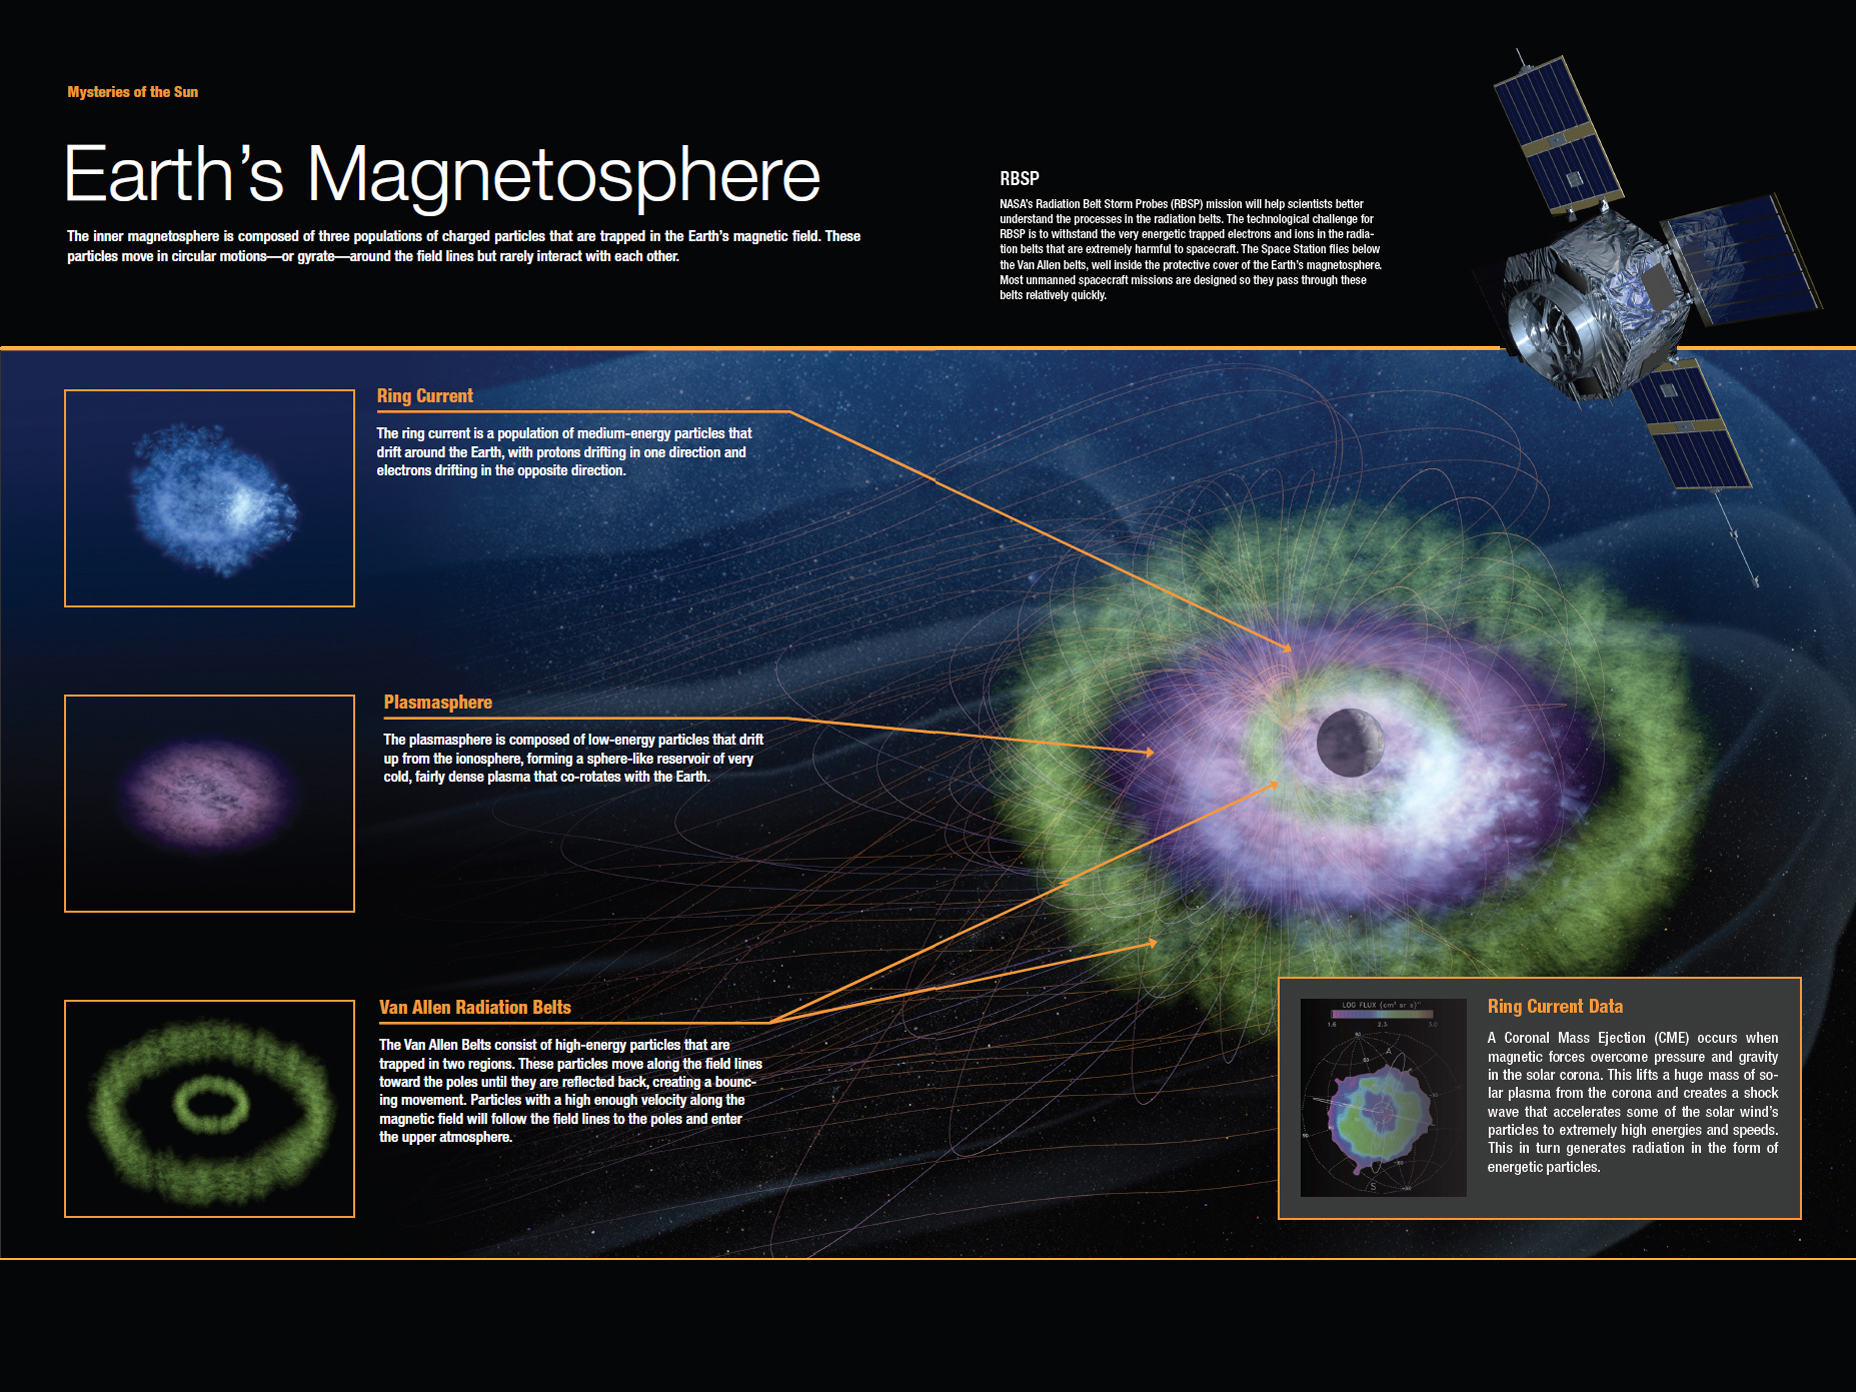
\includegraphics[scale=0.2]{{Figures/innermag.jpg}}
  \caption[Inner Magnetosphere]{Inner Magnetosphere \cite{InnerMagNASA}.}

  % This adds separation space between this figure and either another figure, or between
  %     the figure and the text.
  \figSpace
\end{figure}


\begin{table}
  \centering
  \caption{A table}
  % Tabular environment goes AFTER the caption!
  \begin{tabular}{|c|c|c|}
    % after \\: \hline or \cline{col1-col2} \cline{col3-col4} ...
    \hline
    A & B & C \\\hline
    D & E & F \\\hline
    G & H & I \\
    \hline
  \end{tabular}

  % This adds separation space between this table and either another table, or between
  %     the table and the text.
  \tableSpace
\end{table}
